\chapter{TASK\_1.}

\textbf{Цель работы:}

\begin{itemize} 
	\item Изучить fs, readline-sync и express;
	\item Написать программы, для демонстрации изученного материала;
	\item Научиться взаимодействовать с пользователем через консоль;
	\item Изучить и реализовать работу с файлами;
	\item Изучить формат JSON и научиться работать с ним.
\end{itemize}

\textbf{Задание 1}

С клавиатуры считывается число N. Далее считывается N строк. Необходимо создать массив и сохранять в него строки только с четной длинной. Получившийся массив необходимо преобразовать в строку JSON и сохранить в файл.

\textbf{Задание 2}

Необходимо считать содержимое файла, в котором хранится массив строк в формате JSON. Нужно вывести только те строки на экран, в которых содержатся только гласные буквы.

\textbf{Задание 3}

С клавиатуры считывается строка - название расширения файлов. Далее считывается строка - адрес папки. Необходимо перебрать все файлы в папке и вывести содержимое файлов, у которых расширение совпадает с введенным расширением.

\textbf{Задание 4}

Дана вложенная структура файлов и папок. Все файлы имеют раширение "txt". Необходимо рекурсивно перебрать вложенную структуру и вывести имена файлов, у которых содержимое не превышает по длине 10 символов.

\textbf{Задание 5}

С клавиатуры считывается число N. Далее считывается N строк - имена текстовых файлов. Необходимо склеить всё содержимое введенных файлов в одну большую строку и сохранить в новый файл.

\textbf{Задание 6}

Написать код, который позволяет определить максимальный возможный уровень вложенности друг в друга полей в объекте, чтобы данный объект можно было преобразовать в строку формата JSON. Ответом является целое число.

\textbf{Задание 7}

Из файла считывается строка в формате JSON. В этой строке информация об объекте, в котором находится большое количество вложенных друг в друга полей. Объект представляет из себя дерево. Необходимо рекурсивно обработать дерево и найти максимальную вложенность в дереве. Необходимо вывести на экран ветку с максимальной вложенностью.


\begin{lstlisting}[caption=Код программы. TASK\_1. Главнвая функция main]
	"use strict";

	const readlineSync = require('readline-sync');
	
	const tasks = require("./tasks");
	const constants = require("./constants");
	
	function main() {
		console.log(constants.TASKS_TEXT)
		const answer = readlineSync.question(constants.GREEN + "\n\nTask: ");
	
		if (answer > 7 || answer < 1) {
			console.log(constants.RED + "Error. Bad number.")
			return;
		}
	
		tasks['task' + answer]()
	}
	
	main();
\end{lstlisting}

\begin{lstlisting}[caption=Код программы. TASK\_1. Реализация заданий]
	"use strict";

	const readlineSync = require('readline-sync');
	const fs = require("fs");
	const { deflate } = require('zlib');
	
	function task1() {
		const FILE_NAME = "data/task1.txt";
	
		const N = readlineSync.question("Input N: ");
		const arr = [];
		let line;
	
		for (let i = 0; i < N; i++) {
			line = readlineSync.question("Input str: ");
			if (!(line.length & 1))
				arr.push(line);
		}
	
		// Первый параметр(swedishFamilyObj) - значение, преобразуемое в строку JSON
		// Второй параметр(null) - запрещает замены
		// Третий параметр(4) - размер отступов
		const jsonStr = JSON.stringify(arr, null, 4);
	
		fs.writeFileSync(FILE_NAME, jsonStr);
	}
	
	function countVowels(str) {
		const vowels = 'aeiou';
		let count = 0;
		let arr = str.toLowerCase().split('');
	
		for (let i = 0; i < arr.length; i++) {
			if (vowels.indexOf(arr[i]) !== -1) {
				count++;
			}
		}
	
		return count;
	}
	
	function task2() {
		const FILE_NAME = "data/task2.txt";
	
		const contentFile = fs.readFileSync(FILE_NAME, "utf-8");
		const obj = JSON.parse(contentFile);
	
		console.log("File:" + contentFile);
		console.log("Result:");
		for (let i = 0; i < obj.length; i++) {
			if (countVowels(obj[i]) === obj[i].length)
				console.log(obj[i]);
		}
	}
	
	function task3() {
		// Расширение файлов.
		const extension = readlineSync.question("Input extension: ");
		// Имя папки.
		const folder = readlineSync.question("Input the folder's name: ");
	
		let files;
	
		if (!fs.existsSync(folder)) {
			console.log("Error!\nThe folder does not exist!");
			return;
		}
	
		files = fs.readdirSync(folder);
	
		for (let i = 0; i < files.length; i++) {
			let file = files[i].split('.');
			if (file[file.length - 1] === extension) {
				let contentFile = fs.readFileSync(folder + "/" + files[i], "utf-8");
				console.log(contentFile);
			}
		}
	}
	
	function recursionTask(folder) {
		// По заданию сказано, что все файлы в формате txt
		// Если будут файлы с другим форматом, то сломается программа.
		// (потому что рекурсивная функция попытается открыть этот файл, так
		// как будет думать: 'всё что не txt - значит папка').
		if (!fs.existsSync(folder)) {
			console.log("Error!\nFolder does not exist!");
			return;
		}
	
		let files = fs.readdirSync(folder);
		let contentFile;
	
		for (let i = 0; i < files.length; i++) {
			let file = files[i].split('.');
			if (file[file.length - 1] === "txt") {
				contentFile = fs.readFileSync(folder + "/" + files[i], "utf-8");
				if (contentFile.length < 11) {
					console.log("Path: ", folder + "/" + files[i]);
				}
				// console.log(contentFile, "\n");
			}
			else {
				recursionTask(folder + "/" + files[i]);
			}
		}
	}
	
	function task4() {
		const folder = readlineSync.question("Input the folder's name: ");
		recursionTask(folder);
	}
	
	function task5() {
		const FILE_NAME = "data/task5.txt"
		const N = readlineSync.question("Input N: ");
		let name;
	
		// Очищаем старое содержимое файла (если было)
		fs.writeFileSync(FILE_NAME, "");
		for (let i = 0; i < N; i++) {
			name = readlineSync.question("Input str: ");
			if (!fs.existsSync(name)) {
				console.log("Error!\nThe folder does not exist!");
				return;
			}
			let contentFile = fs.readFileSync(name, "utf-8");
			fs.appendFileSync(FILE_NAME, contentFile);
		}
	}
	
	function task6() {
		// result: 6978
		let a = 1;
		let cnt = 0;
		try {
			while (JSON.stringify(a)) {
				cnt++;
				a = { a };
			}
		} catch (err) {
			console.log(cnt);
		}
	}
	
	
	function find_max_branch(obj, data) {
		if (typeof (obj) !== "object") {
			return;
		}
	
		if (data.curr_depth > data.max_depth)
			data.max_depth = data.curr_depth;
	
		data.curr_depth++;
	
		for (let field in obj) {
			console.log(field)
			data.max_branch.push(field)
			data.max_branch.pop();
			find_max_branch(obj[field], data)
		}
	
		data.curr_depth--;
	}
	
	function task7() {
		let data = {
			"max_branch": [],
			"curr_depth": 0,
			"max_depth": 0
		}
		// data/task7.txt
		// const file_name = readlineSync.question("Input file name: ");
		const file_name = "data/task7.txt";
		const jsonString = fs.readFileSync(file_name, "utf-8");
	
		console.log("FILE:", jsonString)
	
		const obj = JSON.parse(jsonString);
		// console.log(obj);
	
		find_max_branch(obj, data);
		console.log(data)
	}
	
	module.exports = { task1, task2, task3, task4, task5, task6, task7 };
\end{lstlisting}


\textbf{Вывод:}

\begin{itemize} 
	\item Были изучены fs, readline-sync и express;
	\item Были написаны программы, для демонстрации изученного материала;
	\item Было изучено и реализовано взаимодействие с пользователем через консоль;
	\item Было изучено и реализована работа с файлами;
	\item Был изучен формат JSON, а также реализована работа с ним.
\end{itemize}

\textbf{Пример работы:}

\begin{figure}[ht!]
	\centering{
		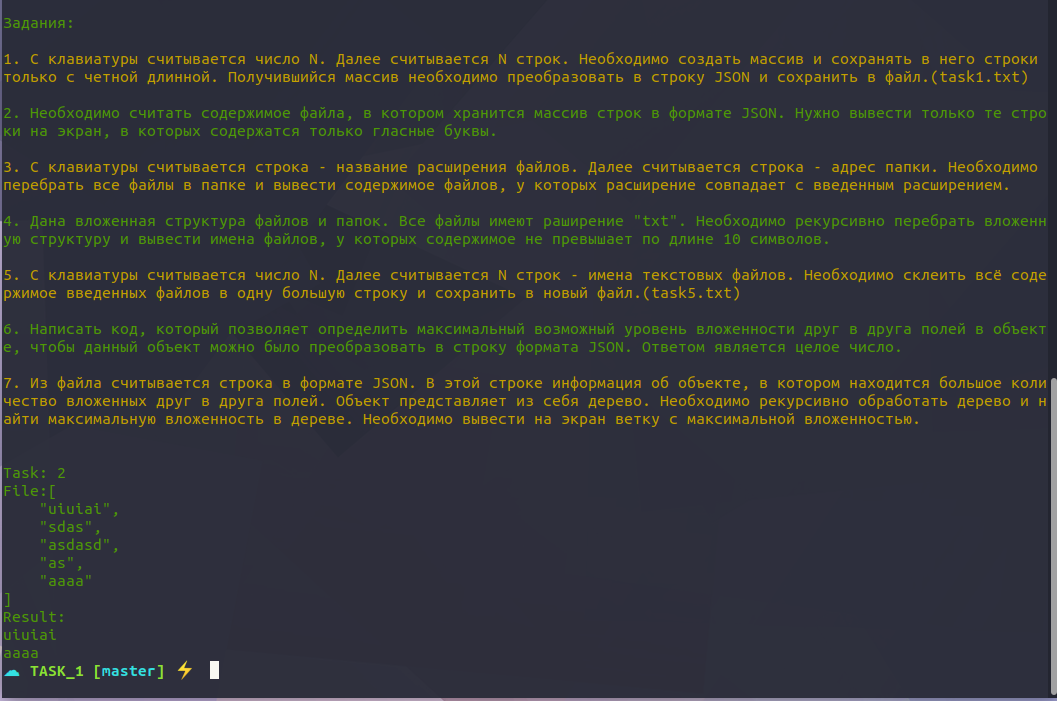
\includegraphics[width=0.9\textwidth]{img/1.png}
		\caption{Пример работы программы}}
\end{figure}

\begin{figure}[ht!]
	\centering{
		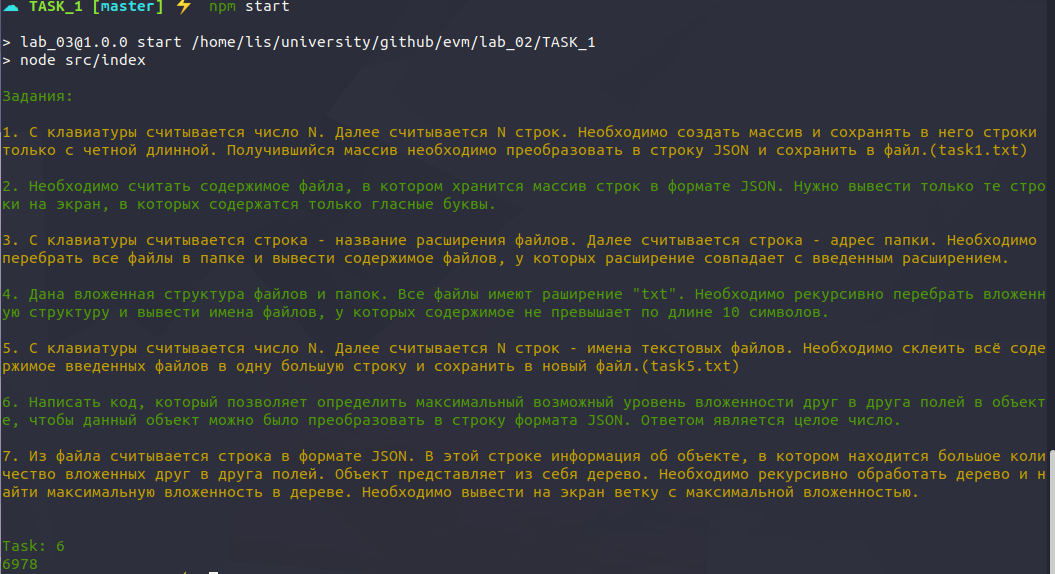
\includegraphics[width=0.9\textwidth]{img/2.png}
		\caption{Пример работы программы}}
\end{figure}

\chapter{TASK\_2.}

\textbf{Цель работы:}

\begin{itemize} 
	\item Научиться запускать собственные сервера;
	\item Изучить и реализовать хранение данных на стороне сервера;
	\item Реализовать генерацию HTML страниц;
	\item Изучить и реализовать взаимодействие с пользователем.
\end{itemize}

\textbf{Задание 1}

Запустить сервер. Реализовать на сервере функцию для сравнения трёх чисел и выдачи наибольшего из них. Реализовать страницу с формой ввода для отправки запроса на сервер.

\textbf{Задание 2}

Запустить сервер. На стороне сервера должен храниться файл, внутри которого находится JSON строка. В этой JSON строке хранится информация о массиве объектов. Реализовать на сервере функцию, которая принимает индекс и выдает содержимое ячейки массива по данному индексу. Реализовать страницу с формой ввода для отправки запроса на сервер.

\textbf{Задание 3}

Написать программу, которая на вход получает массив названий полей и адрес запроса (куда отправлять). Программа должна генерировать HTML разметку страницы, в которую встроена форма для отправки запроса.

\textbf{Задание 4}

Запустить сервер. Реализовать на сервере функцию, которая принимает на вход числа A, B и C. Функция должна выдавать массив целых чисел на отрезке от A до B, которые делятся на C нацело.

\begin{lstlisting}[caption=Код программы. TASK\_2. Реализация заданий]
	const fs = require("fs");

	const ENCODING = "utf-8"
	
	const path = require("path");
	
	function LoadPage(app, path, file_name) {
		app.get(path, (request, response) => {
			const fileContent = fs.readFileSync("public/" + file_name, ENCODING);
			response.end(fileContent);
		});
	}
	
	function task1(app) {
		LoadPage(app, "/compare", "compare.html");
	
		app.get("/compare/result", (request, response) => {
			const a = request.query.a;
			const b = request.query.b;
			const c = request.query.c;
	
			const aInt = parseInt(a);
			const bInt = parseInt(b);
			const cInt = parseInt(c);
	
			if (!aInt || !bInt || !cInt) {
				response.end("Input error!");
				return;
			}
	
			const sInt = Math.max(aInt, bInt, cInt);
	
			response.end("Maximum number: " + sInt);
		});
	}
	
	function task2(app) {
		LoadPage(app, "/array_object", "array_object.html");
	
		app.get("/array_object/result", (request, response) => {
			const index = request.query.index;
			const indexInt = parseInt(index);
			if (!indexInt) {
				response.end("Input error!");
				return;
			}
	
			const PATH = path.join(__dirname, "..", "data", "task2.json");
	
			const array = JSON.parse(fs.readFileSync(PATH));
	
			if (indexInt < 0 || indexInt > array.length) {
				response.end("Index input error!");
				return;
			}
	
			response.end("Index = " + indexInt + "\nelement = " + array[indexInt - 1]);
		});
	}
	
	function task3(app) {
		LoadPage(app, "/generate_html", "generate_html.html");
	
		app.get("/generate_html/result", (request, response) => {
			const field_names = request.query.field_names;
			const address = request.query.address;
			const field_names_array = field_names.split(' ');
	
			const pathBegin = path.join(__dirname, "..", "data", "begin.txt");
			const pathEnd = path.join(__dirname, "..", "data", "end.txt");
	
			const fileBegin = fs.readFileSync(pathBegin, ENCODING)
			const fileEnd = fs.readFileSync(pathEnd, ENCODING)
	
			let fileContent = `<form method="GET" action="${address}">\n`
			for (let i = 0; i < field_names_array.length; i++) {
				fileContent += `
	<p>Введите ${field_names_array[i]}</p>\n\
	<input name="${field_names_array[i]}" spellcheck="false" autocomplete="off"></input>`
			}
	
			fileContent += '\
	<p><button type="submit">Отправить</button></p>\n\
	</form>\n'
	
			response.end(fileBegin + fileContent + fileEnd);
		});
	
	}
	
	function task4(app) {
		LoadPage(app, "/number_array", "number_array.html");
	
		app.get("/number_array/result", (request, response) => {
			const a = request.query.a;
			const b = request.query.b;
			const c = request.query.c;
	
			const aInt = parseInt(a);
			const bInt = parseInt(b);
			const cInt = parseInt(c);
	
			if (!aInt || !bInt || !cInt) {
				response.end("Input error!");
				return;
			}
	
			if (cInt < 0) {
				response.end("C must be positive!");
				return;
			}
	
			let result = "";
			for (let num = aInt; num <= bInt; num++) {
				if (!(num % cInt)) {
					result = result + num + " ";
				}
			}
	
			response.end(result);
		});
	}
	
	
	module.exports = { task1, task2, task3, task4, LoadPage }; //, PATH };
\end{lstlisting}

\begin{lstlisting}[caption=Код программы. TASK\_2. Главная страница]
	<!DOCTYPE html>
	<html lang="ru">
	
	<head>
		<meta charset="UTF-8">
		<link rel="stylesheet" type="text/css" href="../task1.css">
		<title>Выбор задания</title>
	</head>
	
	<body>
		<div id="header">
			<!-- <h1 class="header-title">Выбор задания</h1> -->
			<br>
		</div>
	
		<div id="main">
	
			<h2>Найти наибольшее среди трех чисел</h2>
			<form method="GET" action="/compare/">
				<p><button type="submit">Ввести значения</button></p>
				<!-- <input type="submit" value="Ввести значения"> -->
			</form>
	
			<h2>Получить значение массива по индексу</h2>
			<form method="GET" action="/array_object/">
				<p><button type="submit">Ввести индекс</button></p>
				<!-- <input type="submit" value="Ввести индекс"> -->
			</form>
	
			<h2>Получить разметку</h2>
			<form method="GET" action="/generate_html/">
				<p><button type="submit">Ввести массив названий полей и адрес запроса</button></p>
				<!-- <input type="submit" value="Ввести массив названий полей и адрес запроса "> -->
			</form>
	
			<h2>Получить массив чисел</h2>
			<form method="GET" action="/number_array/">
				<p><button type="submit">Ввести числа A, B и C</button></p>
				<!-- <input type="submit" value="Ввести числа A, B и C"> -->
			</form>
	
		</div>
	</body>
	
	</html>
\end{lstlisting}

\begin{lstlisting}[caption=Код программы. TASK\_2. Страница с заданием 1]
	<!DOCTYPE html>
<!-- <html lang="ru"> -->

<head>
	<meta charset="UTF-8">
	<link rel="stylesheet" type="text/css" href="../task1.css">
	<title>Максимум</title>
</head>

<body>
	<div id="header">
		<!-- <h1 class="header-title">Максимальное число!</h1> -->
	</div>

	<div id="main">

		<h2>Найти наибольшее среди трех чисел</h2>
		<form method="GET" action="/compare/result">
			<p>Введите A</p>
			<input name="a" spellcheck="false" autocomplete="off">
			<p>Введите B</p>
			<input name="b" spellcheck="false" autocomplete="off">
			<p>Введите C</p>
			<input name="c" spellcheck="false" autocomplete="off">
			<br>
			<br>
			<p><button type="submit">Найти наибольшее</button></p>
			<!-- <input type="submit" value="Найти наибольшее"> -->
		</form>

	</div>
</body>

</html>
\end{lstlisting}


\begin{lstlisting}[caption=Код программы. TASK\_2. Страница с заданием 2]
	<!DOCTYPE html>
<!-- <html lang="ru"> -->

<head>
	<meta charset="UTF-8">
	<link rel="stylesheet" type="text/css" href="../task1.css">
	<title>Элемент массива</title>
</head>

<body>
	<div id="header">
		<!-- <h1 class="header-title">Элемент массива!</h1> -->
	</div>

	<div id="main">
		<h2>Получить значение массива по индексу</h2>
		<form method="GET" action="/array_object/result">
			<p>Индекс</p>
			<input name="index" spellcheck="false" autocomplete="off">
			<br>
			<br>
			<p><button type="submit">Получить</button></p>
			<!-- <input type="submit" value="Получить"> -->
		</form>

	</div>
</body>

</html>
\end{lstlisting}


\begin{lstlisting}[caption=Код программы. TASK\_2. Страница с заданием 3]
	<!DOCTYPE html>
<!-- <html lang="ru"> -->

<head>
	<meta charset="UTF-8">
	<link rel="stylesheet" type="text/css" href="../task1.css">
	<title>Генерация страницы</title>
</head>

<body>
	<div id="header">
		<!-- <h1 class="header-title">Генерация разметки!</h1> -->
	</div>

	<div id="main">
		<h2>Получить разметку страницы</h2>
		<form method="GET" action="/generate_html/result">
			<p>Название полей</p>
			<input name="field_names" spellcheck="false" autocomplete="off">
			<p>адрес</p>
			<input name="address" spellcheck="false" autocomplete="off">
			<br>
			<br>
			<p><button type="submit">Получить</button></p>
			<!-- <input type="submit" value="Получить"> -->
		</form>

	</div>
</body>

</html>
\end{lstlisting}


\begin{lstlisting}[caption=Код программы. TASK\_2. Страница с заданием 4]
	<!DOCTYPE html>

<head>
	<meta charset="UTF-8">
	<link rel="stylesheet" type="text/css" href="../task1.css">
	<title>Массив</title>
</head>

<body>
	<div id="header">
		<!-- <h1 class="header-title">Массив!</h1> -->
	</div>

	<div id="main">
		<h2>Получить массив целых чисел на отрезке от A до B, которые делятся на C нацело.</h2>
		<form method="GET" action="/number_array/result">
			<p>Введите A</p>
			<input name="a" spellcheck="false" autocomplete="off">
			<p>Введите B</p>
			<input name="b" spellcheck="false" autocomplete="off">
			<p>Введите C</p>
			<input name="c" spellcheck="false" autocomplete="off">
			<br>
			<br>
			<p><button type="submit">Получить массив</button></p>
			<!-- <input type="submit" value="Получить массив"> -->
		</form>

	</div>
</body>

</html>
\end{lstlisting}

\begin{lstlisting}[caption=Код программы. TASK\_2. Стили страницы]
	* {
		box-sizing: border-box;
		color: #FFC0CB;
		text-align: center;
	}
	h2 {
		color: #FFC0CB;
	
	}
	
	p {
		font-size: 30px;
	
	}
	
	:root {
		--background: #E0FFFF;
		--background-accent: #FFC0CB;
		--background-accent-2: #FFFFFF;
		--light: #FFFFFF;
		--dark: #E0FFFF;
		--text: #C8A2C8
	}
	
	body {
		  background-color: var(--background);
		background-image: linear-gradient(
			var(--background-accent-2) 50%,
			var(--background-accent) 50%
		), linear-gradient(
			var(--background-accent) 50%,
			var(--background-accent-2) 50%
		);
		background-repeat: no-repeat;
		background-size: 100% 30px;
		background-position: top left, bottom left;
		/* min-height: 100vh; */
	}
	
	div {
		display: block;
		width: 400px;
		margin: 0 auto 0 auto;
		position: absolute;
		left: 0;
		right: 0;
		top: 15vh; 
	 }
	
	button {
		display: block;
		cursor: pointer;
		outline: none;
		border: none;
		background-color: var(--light);
		width: 400px;
		height: 70px;
		border-radius: 30px;
		font-size: 1.2rem;
		font-weight: 600;
		color: var(--text);
		background-size: 100% 100%;
		box-shadow: 0 0 0 7px var(--light) inset;
		margin-bottom: 15px;
	
		/* text-shadow: #cad5e2 1px 1px 0, #cad5e2 2px 2px 0, 
				#cad5e2 3px 3px 0, #cad5e2 4px 4px 0, 
				#cad5e2 5px 5px 0; */
	}
	
	button:hover {
		background-image: linear-gradient(
			145deg,
			transparent 10%,
			var(--dark) 10% 20%,
			transparent 20% 30%,
			var(--dark) 30% 40%,
			transparent 40% 50%,
			var(--dark) 50% 60%,
			transparent 60% 70%,
			var(--dark) 70% 80%,
			transparent 80% 90%,
			var(--dark) 90% 100%
		);
		animation: background 3s linear infinite;
	}
	
	input {
		/* border: none; */
		font-size:22px;
		font-family:Tahoma, Geneva, sans-serif;
		/* color:#000000;   */
		margin:0 0 6px 0;
	}
	
	@keyframes background {
	  0% {
		background-position: 0 0;
	  }
	  100% {
		background-position: 400px 0;
	  }
	}
\end{lstlisting}


\textbf{Вывод:}

\begin{itemize} 
	\item Мы запустили собственные сервера;
	\item Мы изучили и реализовали хранение данных на стороне сервера;
	\item Реализовали генерацию HTML страниц;
	\item Изучили и реализовали взаимодействие с пользователем.
\end{itemize}


\textbf{Пример работы:}

\begin{figure}[ht!]
	\centering{
		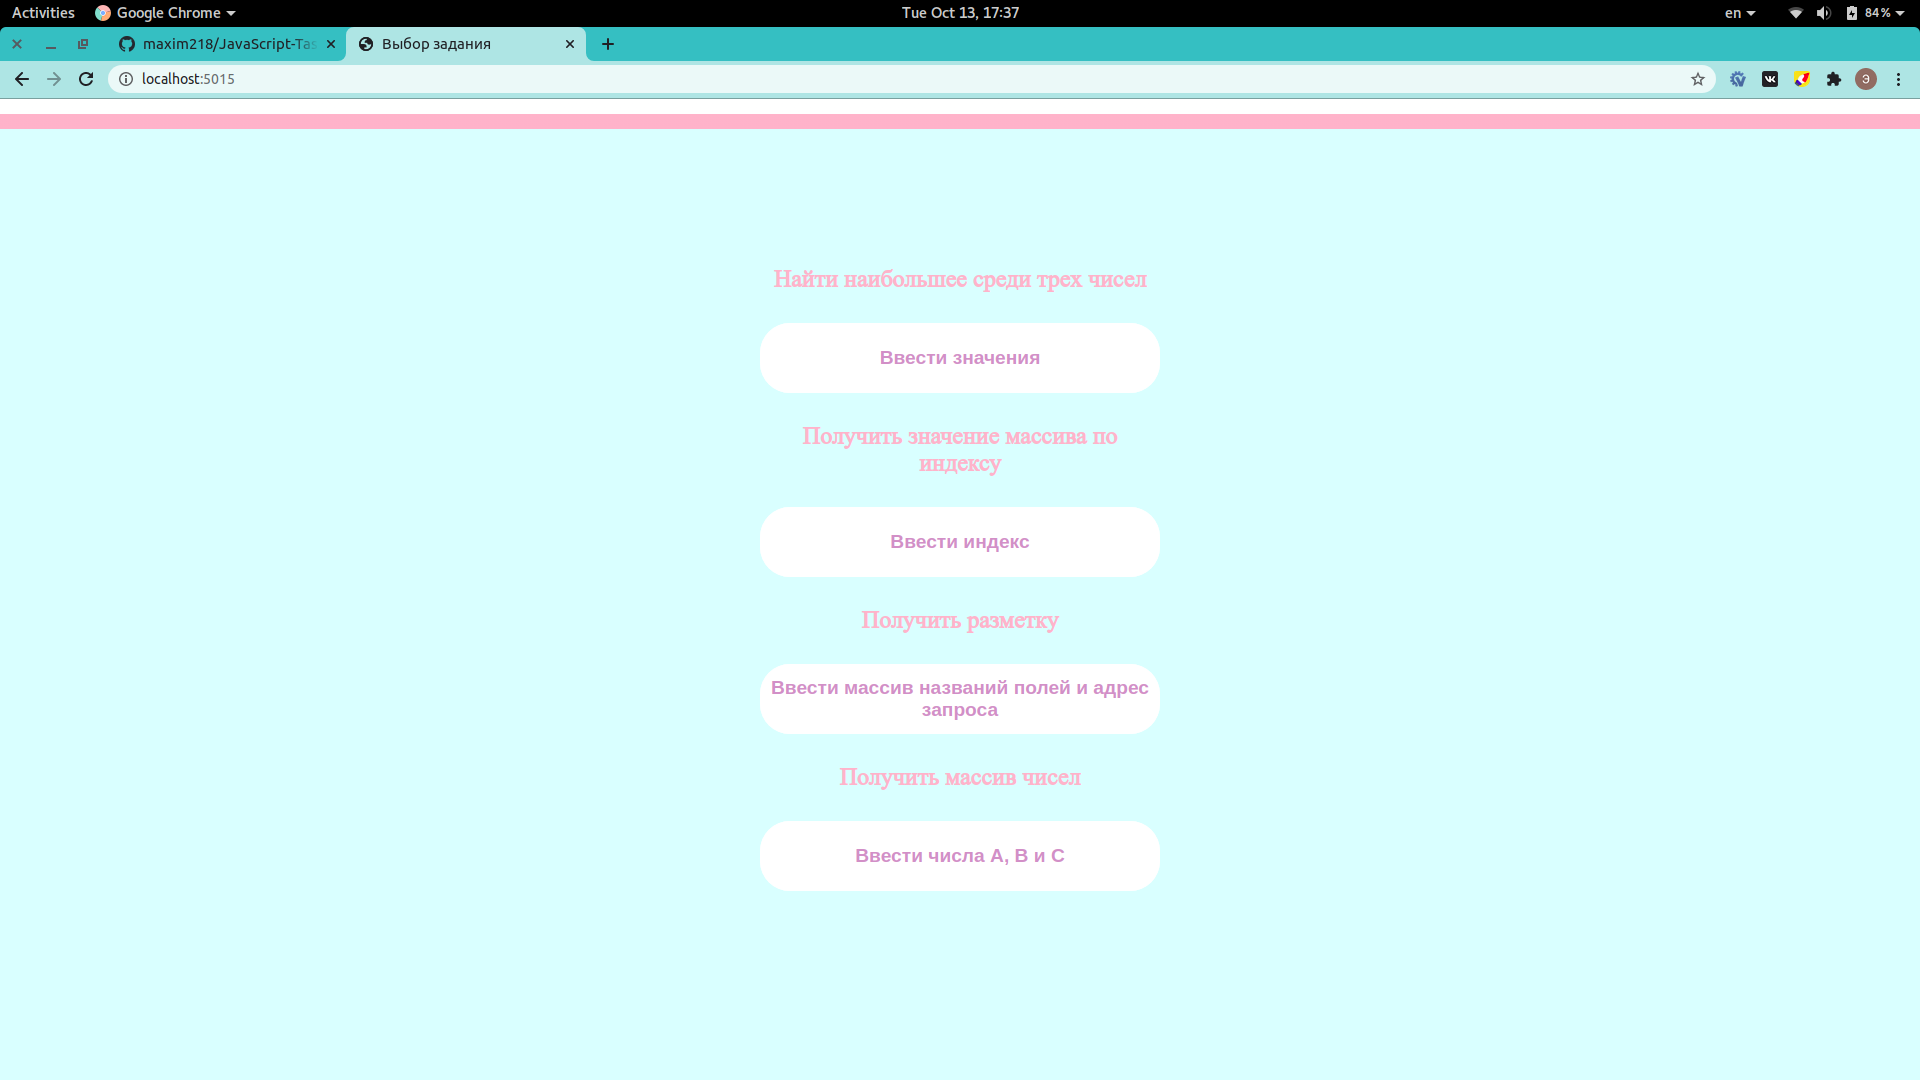
\includegraphics[width=0.9\textwidth]{img/3.png}
		\caption{Пример работы программы}}
\end{figure}

\begin{figure}[ht!]
	\centering{
		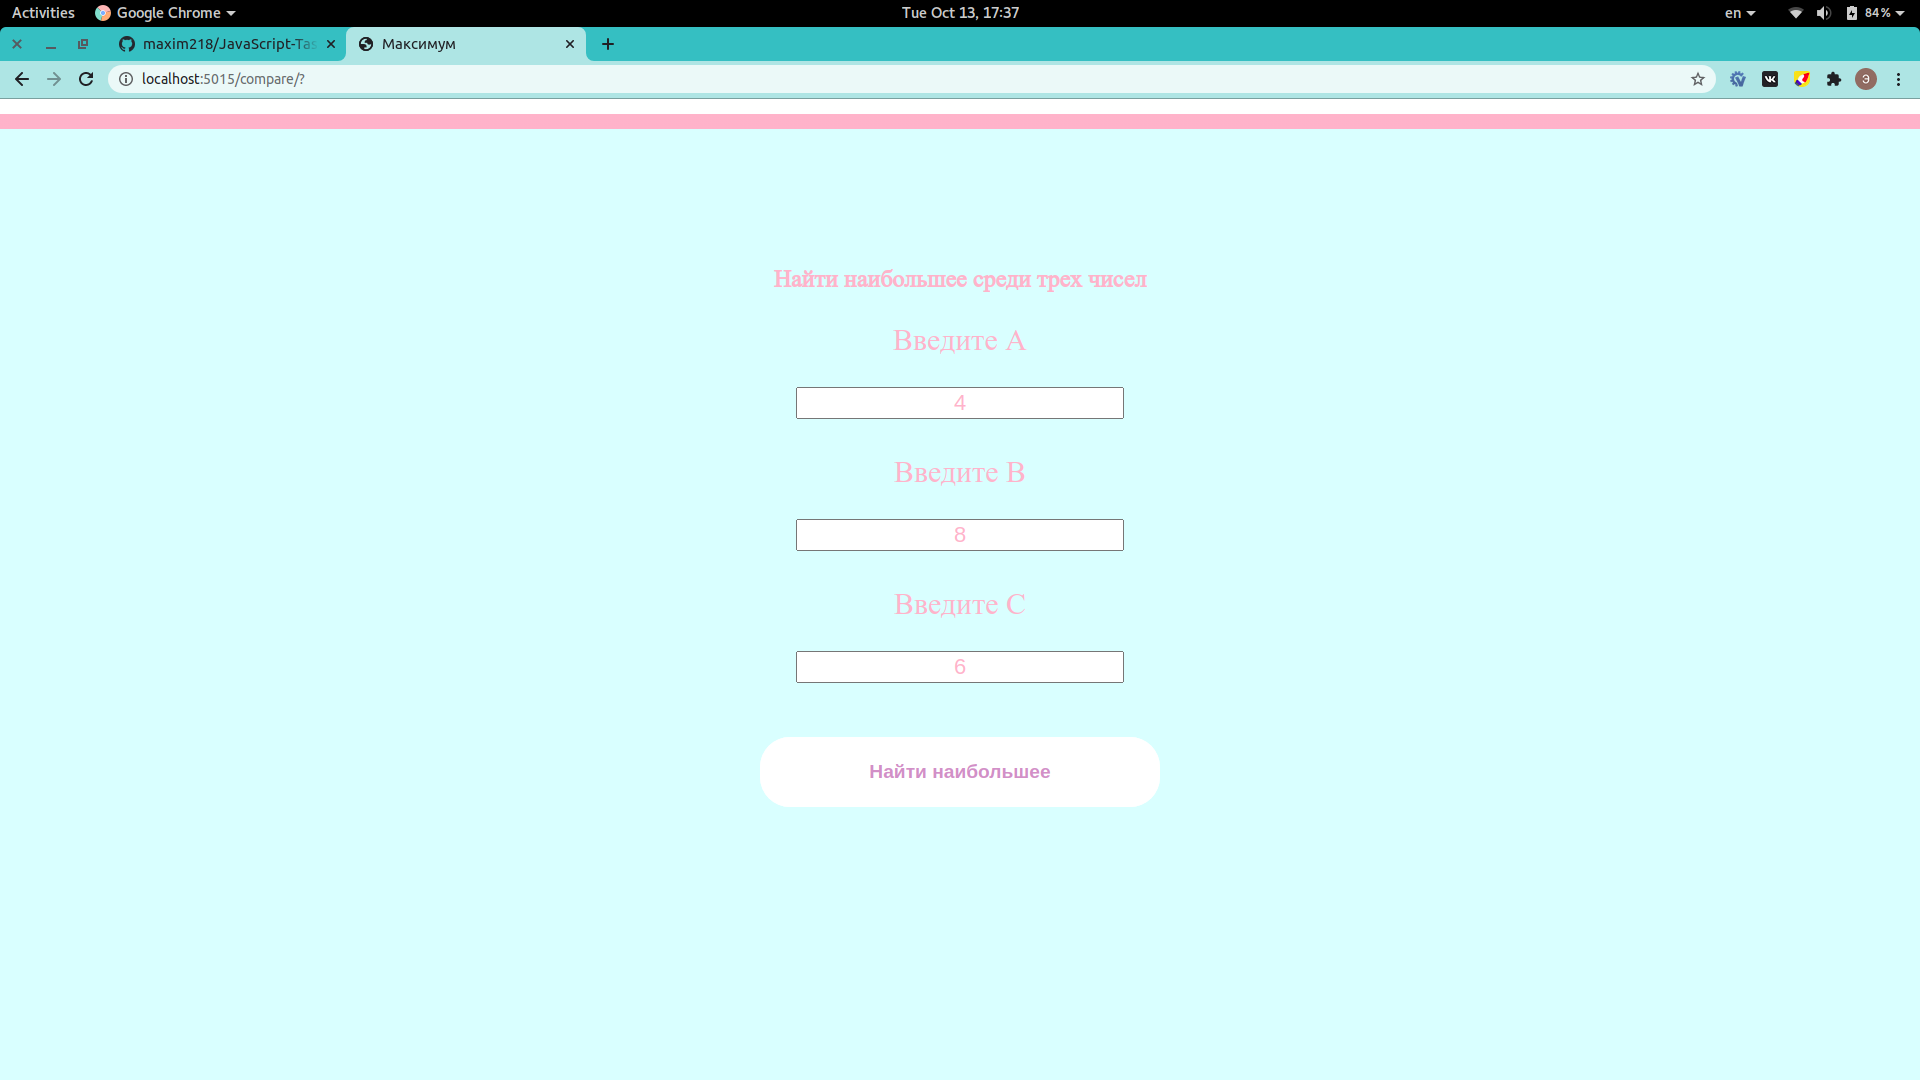
\includegraphics[width=0.9\textwidth]{img/4.png}
		\caption{Пример работы программы}}
\end{figure}

\begin{figure}[ht!]
	\centering{
		
\includegraphics[width=0.9\textwidth]{img/5.png}
		\caption{Пример работы программы}}
\end{figure}

% \begin{figure}[ht!]
% 	\centering{
% 		
\includegraphics[width=0.9\textwidth]{img/6.png}
% 		\caption{Пример работы программы}}
% \end{figure}

\begin{figure}[ht!]
	\centering{
		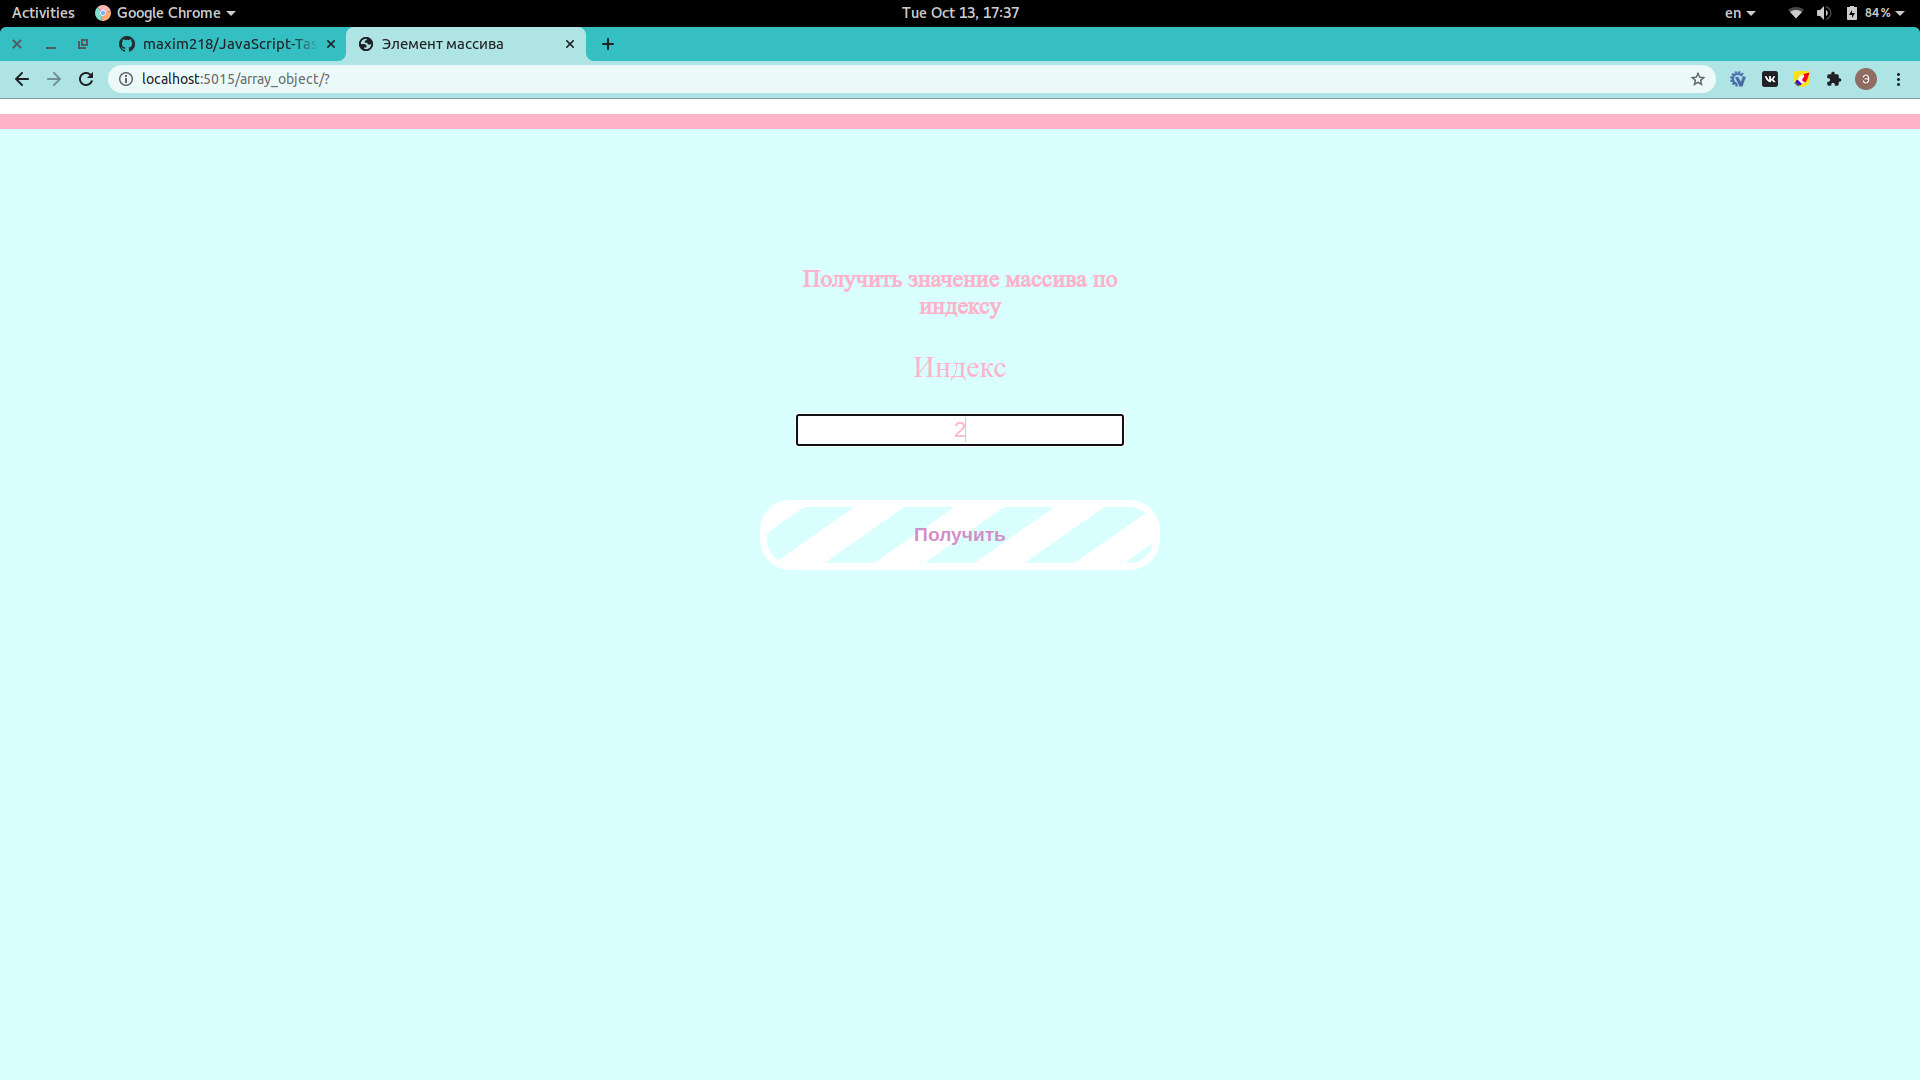
\includegraphics[width=0.9\textwidth]{img/7.png}
		\caption{Пример работы программы}}
\end{figure}

\begin{figure}[ht!]
	\centering{
		
\includegraphics[width=0.9\textwidth]{img/8.png}
		\caption{Пример работы программы}}
\end{figure}

\begin{figure}[ht!]
	\centering{
		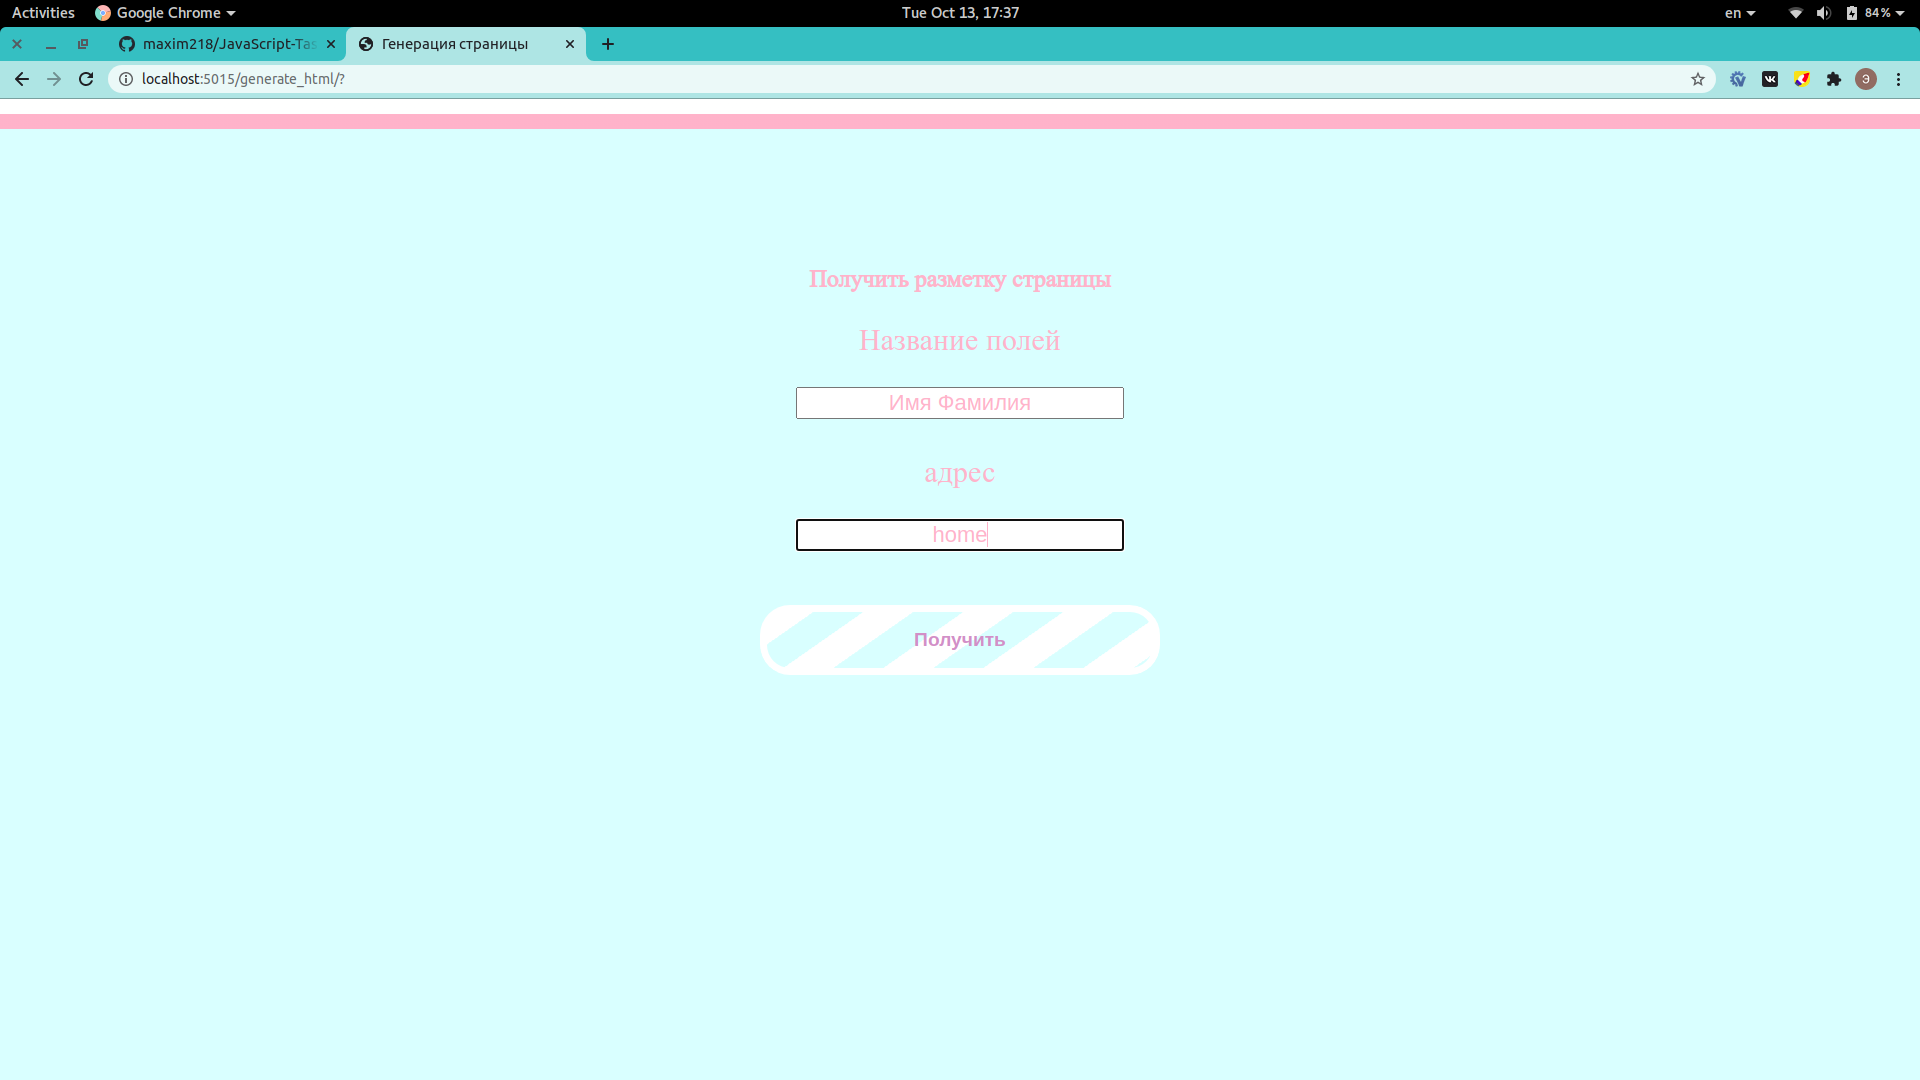
\includegraphics[width=0.9\textwidth]{img/9.png}
		\caption{Пример работы программы}}
\end{figure}

\begin{figure}[ht!]
	\centering{
		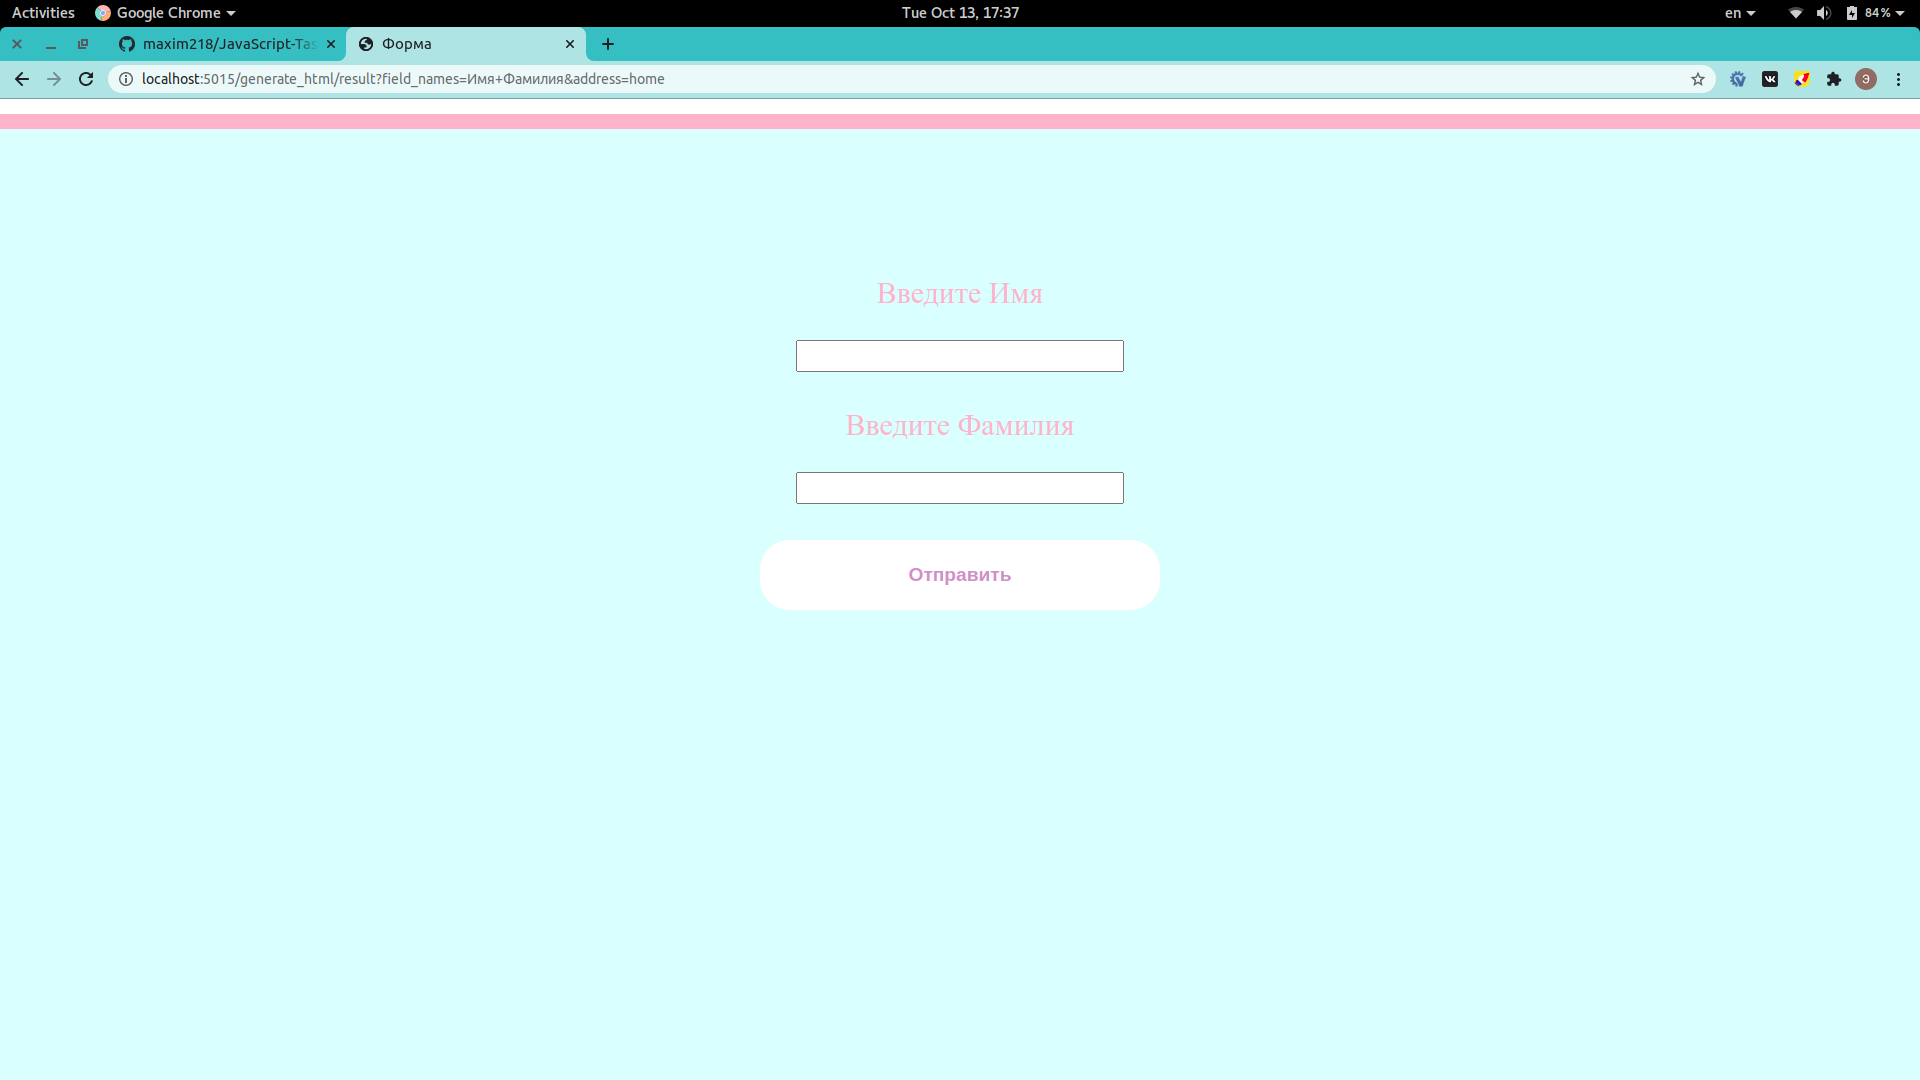
\includegraphics[width=0.9\textwidth]{img/10.png}
		\caption{Пример работы программы}}
\end{figure}

\begin{figure}[ht!]
	\centering{
		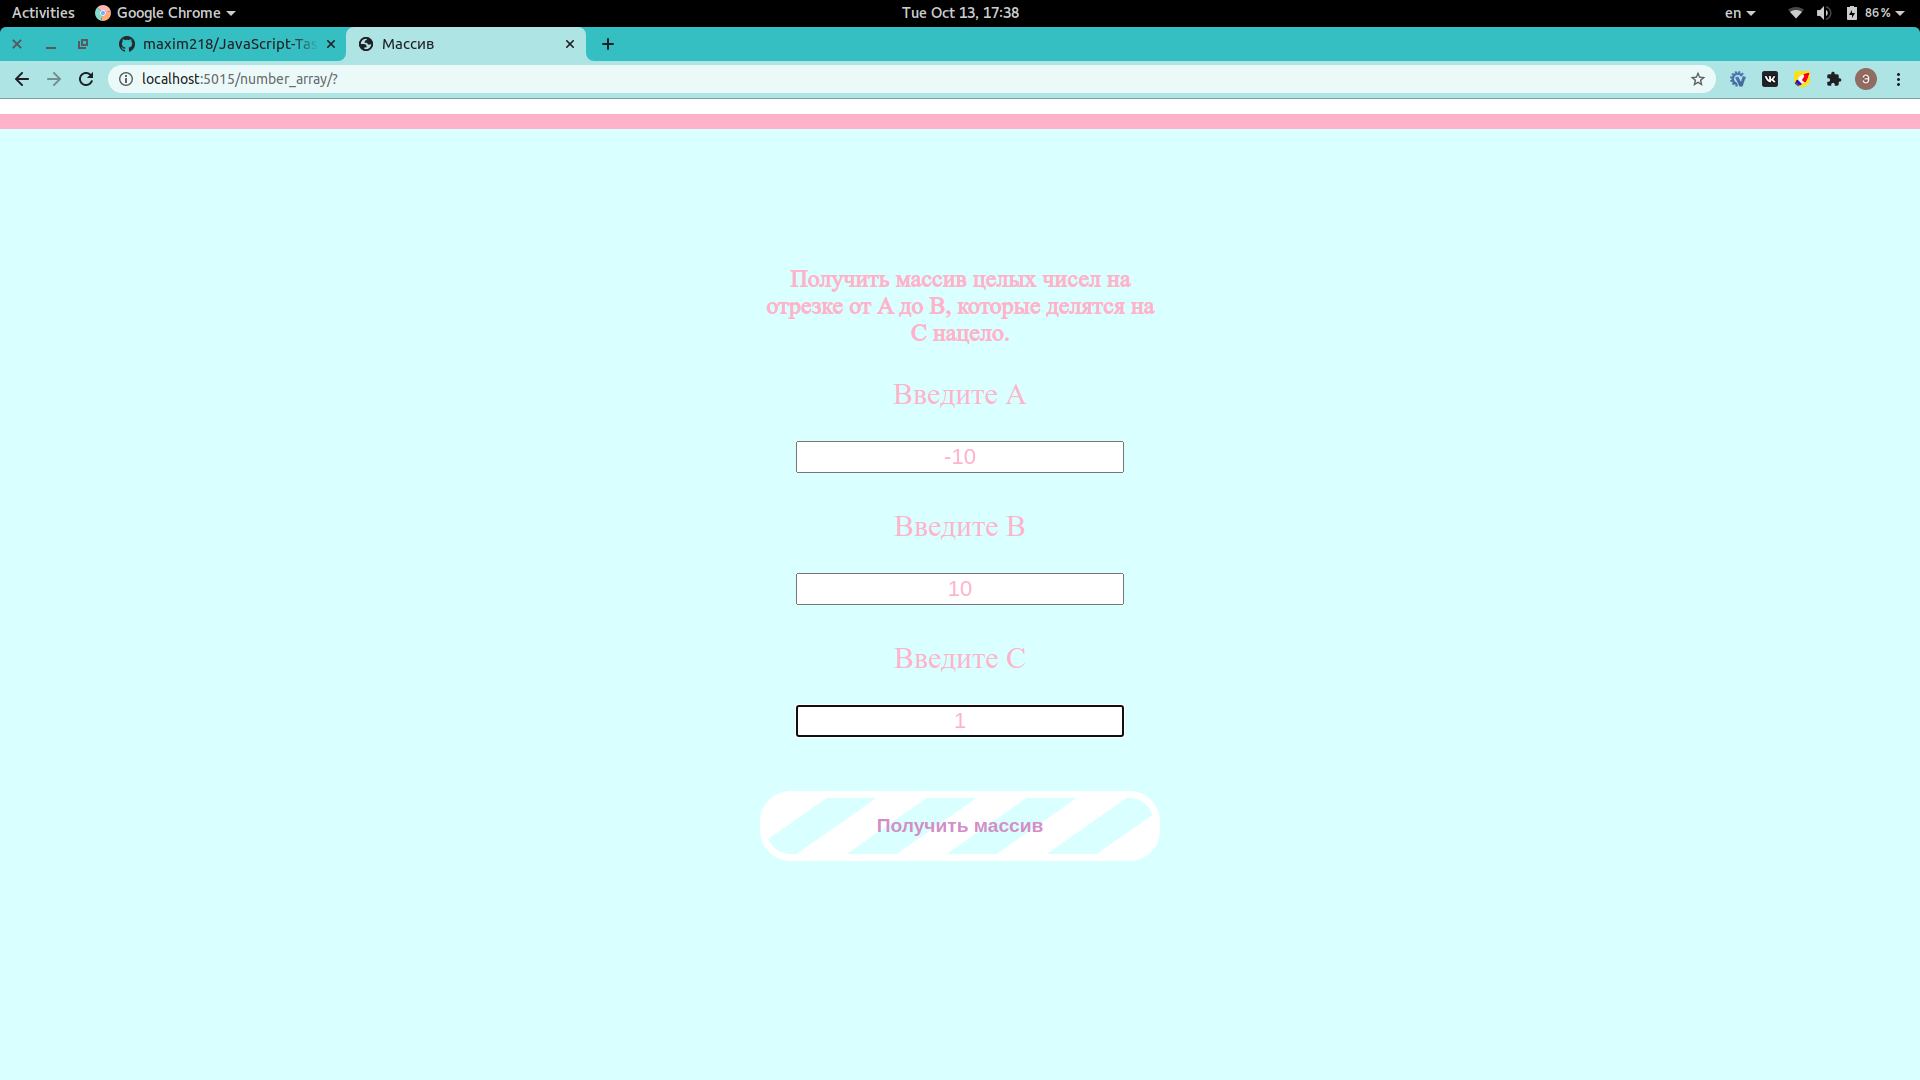
\includegraphics[width=0.9\textwidth]{img/11.png}
		\caption{Пример работы программы}}
\end{figure}

\begin{figure}[ht!]
	\centering{
		
\includegraphics[width=0.9\textwidth]{img/12.png}
		\caption{Пример работы программы}}
\end{figure}
